\documentclass{article}
\usepackage[english]{babel}
\usepackage[letterpaper,top=2cm,bottom=2cm,left=3cm,right=3cm,marginparwidth=1.75cm]{geometry}

\usepackage{amsmath}
\usepackage{amsfonts}

\usepackage{graphicx}
\usepackage{float}
\usepackage[colorlinks=true, allcolors=cyan]{hyperref}


\usepackage{caption}
\usepackage[svgnames]{xcolor}
\usepackage[font={color=White},figurename=Fig.,labelfont={it}]{caption}

\title{Analyzing the Topological Properties of 3D STL Files}
\author{Sahil Dhawan}
\begin{document}

%Commands definitions
\newcommand{\setbackgroundcolor}{\pagecolor[rgb]{0,0,0}}  
\newcommand{\settextcolor}{\color[rgb]{1,1,1}}
\newcommand{\invertbackgroundtext}{\setbackgroundcolor\settextcolor}

%Command execution. 
\invertbackgroundtext


\maketitle
\begin{abstract}
DO THIS LAST
\end{abstract}

\section{Introduction}

DO THIS LAST

\section{Background}

\subsection{simplicial homology}

\cite{Hatcher_2001}

\subsection{persistent homology}

\subsubsection{Cech Complexes}
$Cech_{r}(X) = \{\sigma \subseteq X \mid \cap_{x \in \sigma} B_{r}(X) \not= \emptyset\}$
\begin{itemize}
\item Balls grow around points of metric space, every time k+1 balls intersect, add a k-dimensional simplex to complex.
\end{itemize}

\subsubsection{Vietoris-Rips Complexes}
$VR_{r}(X) = \{\sigma \subseteq X \mid diam\sigma \leq 2r \}$
\begin{itemize}
\item if subsets of metric space have diameter less than or equal to 2*r, add simplex
\end{itemize}

\subsubsection{Delaunay Complexes}
$Del(X) = \{\sigma \subseteq X \mid \cap_{x \in \sigma} V_{x} \not= \emptyset\}$

$V_{x} = \{y \in \mathbb{R}^{2} \mid ||y-x|| \leq  ||y-z||, z \in X\}$
\begin{itemize}
\item Do not depend on a parameter or intersecting balls (no "time")
\item Intersecting voronoi cells determine simplices in complex
\end{itemize}

\subsubsection{Alpha Complexes}
$Alpha_{r}(X)=\{\sigma \subseteq X \mid \cap_{x\in \sigma} (B_{r}(X) \cap V_{x}) \not= \emptyset\}$
\begin{itemize}
\item in-between cech and delauney complexes: to construct, take into account both voronoi cell-associated points in metric spce and growing balls around these points

\end{itemize}
\subsection{Formula}

\section{Methods}

\subsection{What is an STL File?}
An STL file is 

\subsubsection{Converting the .ast File to a Data Structure}

The .ast file was parsed for four strings which are used to denote the beginning and end of the description of faces and vertices: "facet normal", "end facet", "outer loop", and "end loop", respectively. The data was then converted into tuple with python:
$$[[\text{'Face 0'}, [\text{normal vector xyz}],[\text{[point 1 xyz}], [\text{point 2 xyz}], [\text{point 3 xyz}]]], [\text{'Face 1'}, ... ]]$$

\begin{figure}[H]
    \centering
    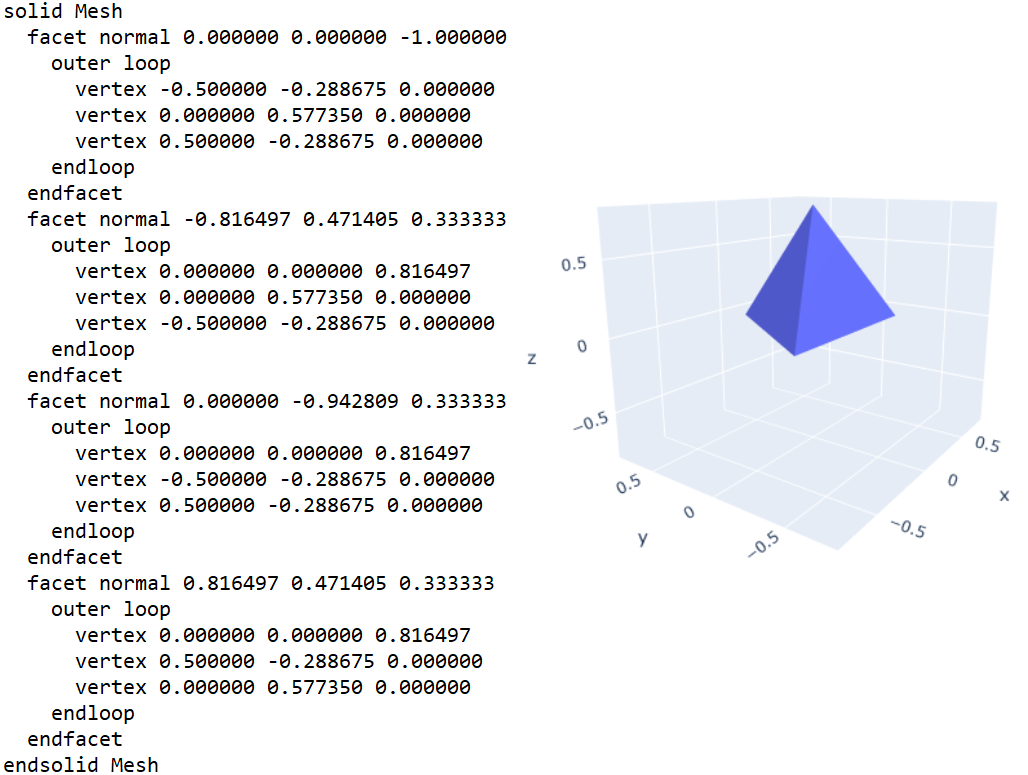
\includegraphics[width=0.5\linewidth]{tetrahedron_ast_code_plot.png}
    \caption{The contents of a .AST file representing the tetrahedron shown on the right.}
    \label{fig:ast_code}
\end{figure}

\subsection{Python Libraries}

\subsection{Meshing}

\subsection{Filtration Construction}

\subsection{Persistence Diagram Construction}

\section{Results}

\section{Discussion}

\section{Conclusion}
DO THIS LAST

\section{Bibliography}
\subsection{How to add Citations and a References List}

\bibliographystyle{alpha}
\bibliography{thesis_bib}

\end{document}
